% Fluxograma metodológico (pipeline de previsão de ocorrência de fogo).
% Compilado à parte (pdflatex fluxograma_pipeline.tex) e incluído no tcc.tex
% como imagem, para não carregar TikZ no documento principal (Overleaf).
\documentclass[tikz,border=4pt]{standalone}
\usepackage[T1]{fontenc}
\usepackage[utf8]{inputenc}
\usepackage{amsmath}
\usepackage[scaled]{helvet}
\renewcommand{\familydefault}{\sfdefault}
\usetikzlibrary{positioning,arrows.meta,fit,backgrounds}

\begin{document}
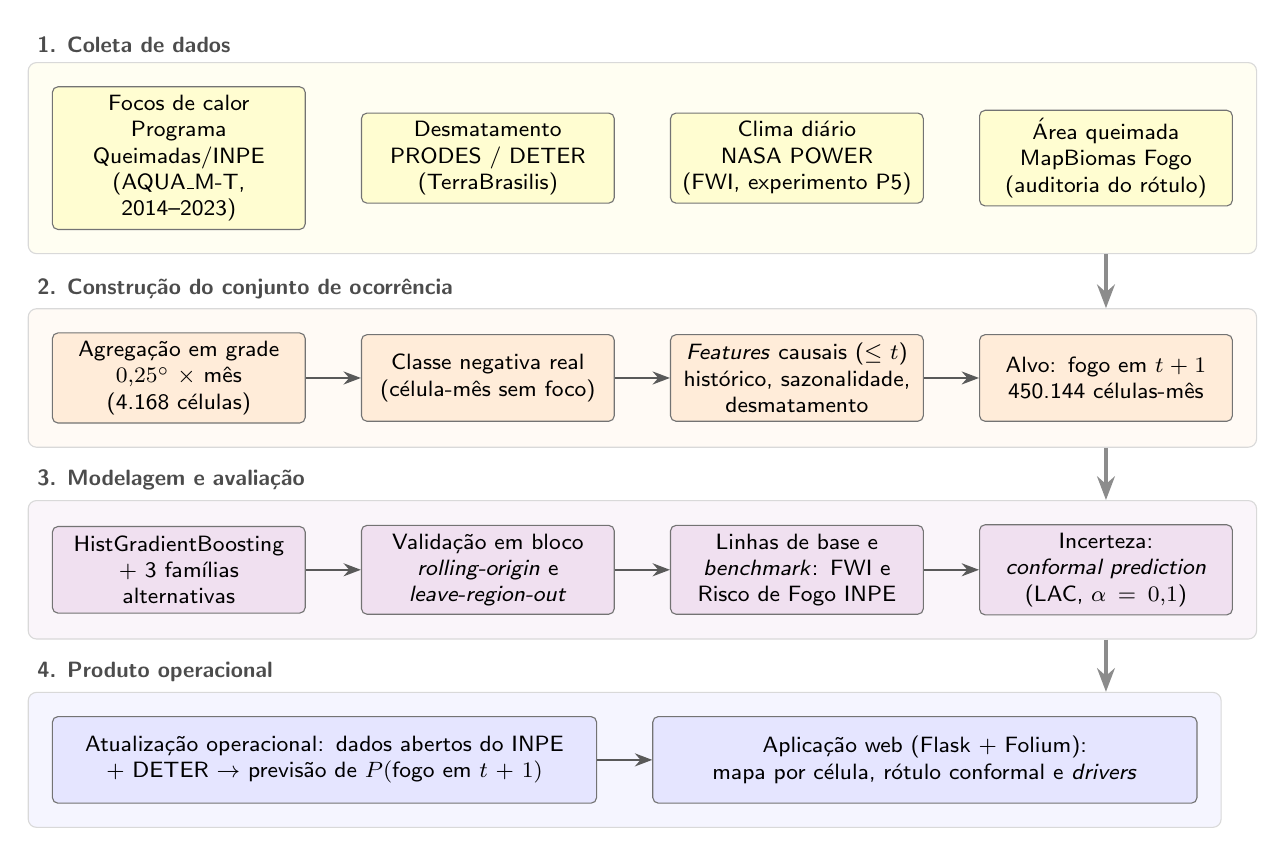
\begin{tikzpicture}[
  node distance=5mm and 7mm,
  box/.style={draw=black!55, rounded corners=2pt, fill=#1, align=center,
              font=\footnotesize, minimum height=11mm, text width=30mm, inner sep=3pt},
  box/.default=white,
  seta/.style={-{Stealth[length=2.2mm]}, thick, black!65},
  fase/.style={font=\footnotesize\bfseries, black!70, anchor=south west},
  faixa/.style={draw=black!15, fill=#1, rounded corners=3pt, inner sep=3mm},
]
% ---- Linha 1: fontes de dados
\node[box=yellow!18] (inpe) {Focos de calor\\ Programa Queimadas/INPE\\ (AQUA\_M-T, 2014--2023)};
\node[box=yellow!18, right=of inpe] (deter) {Desmatamento\\ PRODES / DETER\\ (TerraBrasilis)};
\node[box=yellow!18, right=of deter] (clima) {Clima diário\\ NASA POWER\\ (FWI, experimento P5)};
\node[box=yellow!18, right=of clima] (mapb) {Área queimada\\ MapBiomas Fogo\\ (auditoria do rótulo)};

% ---- Linha 2: construção do conjunto
\node[box=orange!15, below=13mm of inpe] (grade) {Agregação em grade\\ $0{,}25^\circ$ $\times$ mês\\ (4.168 células)};
\node[box=orange!15, right=of grade] (neg) {Classe negativa real\\ (célula-mês sem foco)};
\node[box=orange!15, right=of neg] (feat) {\emph{Features} causais ($\le t$)\\ histórico, sazonalidade,\\ desmatamento};
\node[box=orange!15, right=of feat] (alvo) {Alvo: fogo em $t+1$\\ 450.144 células-mês};

% ---- Linha 3: modelagem e validação
\node[box=violet!12, below=13mm of grade] (modelo) {HistGradientBoosting\\ + 3 famílias\\ alternativas};
\node[box=violet!12, right=of modelo] (valid) {Validação em bloco\\ \emph{rolling-origin} e\\ \emph{leave-region-out}};
\node[box=violet!12, right=of valid] (bench) {Linhas de base e\\ \emph{benchmark}: FWI e\\ Risco de Fogo INPE};
\node[box=violet!12, right=of bench] (conf) {Incerteza:\\ \emph{conformal prediction}\\ (LAC, $\alpha=0{,}1$)};

% ---- Linha 4: produto
\node[box=blue!10, below=13mm of modelo.south west, anchor=north west, text width=67mm] (atual) {Atualização operacional: dados abertos do INPE\\ + DETER $\rightarrow$ previsão de $P(\text{fogo em } t+1)$};
\node[box=blue!10, right=of atual, text width=67mm] (app) {Aplicação web (Flask + Folium):\\ mapa por célula, rótulo conformal e \emph{drivers}};

% ---- Setas (dentro de cada fase)
\draw[seta] (grade) -- (neg);
\draw[seta] (neg) -- (feat);
\draw[seta] (feat) -- (alvo);
\draw[seta] (modelo) -- (valid);
\draw[seta] (valid) -- (bench);
\draw[seta] (bench) -- (conf);
\draw[seta] (atual) -- (app);

% ---- Faixas das fases
\begin{scope}[on background layer]
  \node[faixa=yellow!5, fit=(inpe)(mapb)] (f1) {};
  \node[faixa=orange!4, fit=(grade)(alvo)] (f2) {};
  \node[faixa=violet!4, fit=(modelo)(conf)] (f3) {};
  \node[faixa=blue!4, fit=(atual)(app)] (f4) {};
\end{scope}
\node[fase] at (f1.north west) {1. Coleta de dados};
\node[fase] at (f2.north west) {2. Construção do conjunto de ocorrência};
\node[fase] at (f3.north west) {3. Modelagem e avaliação};
\node[fase] at (f4.north west) {4. Produto operacional};
% ---- Setas entre fases
\foreach \de/\para in {f1/f2, f2/f3, f3/f4}
  \draw[-{Stealth[length=3mm]}, line width=1.6pt, black!45]
    (conf |- \de.south) -- (conf |- \para.north);
\end{tikzpicture}
\end{document}
